%! TEX root = ../../master.tex
\lecture[General matchings via $\LP$. Prerequisites for blossom algorithm.]{Th 02 June 2022}{General matchings}

\subsection{Combinatorial algorithms for $\IP$}
We already considered polynomial algorithms for bipartite matchings, but can we extend this
to general graphs?

\begin{recall}
    We defined a (weighted) matching via $\IP$ as
    \begin{maxi*}{x}{w^Tx}{}{}
        \addConstraint{\sum_{e\in \delta(v)}x_e}{\leq 1, \quad}{\forall v \in V}
        \addConstraint{x}{\in \bool^E}
    \end{maxi*}
    For the linear relaxation, we can find non-bipartite graphs with non-integral optimal solutions.
\end{recall}
\begin{idea}
    To fix the issue of fractional vertices, we want to add cutting planes that cut only these fractional vertices off.
    More general, we want to cut off odd cycles by introducing constraints
    \begin{align*}
        \sum_{e\in E(S)}x_e \leq \left\lfloor \frac{|S|}{2} \right\rfloor
    \end{align*}
    for every $S\subseteq V$ with odd cardinality.
    We will call these \vocab{blossom constraints}.
\end{idea}
\begin{example} \label{ex:non-int-matching}
    For following graph
    \\
    \begin{minipage}{\textwidth}
        \centering
        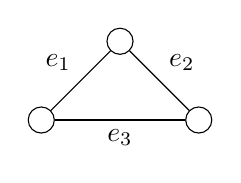
\begin{tikzpicture}
            \begin{scope}[every node/.style={circle, draw}]

                \node (1) at (0,0) {};
                \node (2) at (1,1) {};
                \node (3) at (2,0) {};

            \end{scope}
            \path (1) edge node[anchor=south east] {$e_1$} (2);
            \path (2) edge node[anchor=south west] {$e_2$}(3);
            \path (1) edge node[anchor=north] {$e_3$}(3);
        \end{tikzpicture}
        % \captionof{figure}{A graph with $S$ colored orange}
    \end{minipage}
    is $[0.5, 0.5, 0.5]^T$ an optimal vertex for the $\LP$ relaxation, but introducing
    \begin{align*}
        x_{e_1}+x_{e_2}+x_{e_3} \leq 1
    \end{align*}
    would cut this solution.
\end{example}

\begin{definition}
    Given a graph $G=(N,E)$ and matching $M$.
    \begin{enumerate}
        \item A path is \vocab{alternating} w.r.t. $M$
              if its edges alternate between $M$ and $E-M$.
        \item A node is \vocab{exposed} if no edge in $M$ hits the node.
        \item A path is \vocab{augmenting} if it is alternating and both endpoints are exposed.
    \end{enumerate}
\end{definition}
\begin{theorem}
    A matching $M$ is not maximum iff there exist an augmenting path w.r.t. $M$.
\end{theorem}
\begin{proof}
    The reverse is clear. Thus, consider a non-maximum matching $M$. Then there
    is a matching $M'$ with $|M'|=|M|+1$. Let $D=\textcolor{blue}{M} \Delta \textcolor{orange}{M'}$, then
    $D$ is composed from paths or even-sized cycles only, e.g.
    \vspace{8pt}
    \\
    \begin{minipage}{\textwidth}
        \centering
        \begin{tikzpicture}
            \begin{scope}[every node/.style={circle, draw}]

                \node (1) at (0,0) {};
                \node (2) at (2,0) {};
                \node (3) at (2,2) {};
                \node (4) at (0,2) {};

                \node (a) at (4,0.5) {};
                \node (b) at (5,1.5) {};
                \node (c) at (6,0.5) {};
                \node (d) at (7,1.5) {};
                \node (e) at (8,0.5) {};
                \node (f) at (9,1.5) {};
            \end{scope}
            \path[draw=blue] (1) edge (2);
            \path[draw=blue] (3) edge (4);
            \path[draw=orange] (2) edge (3);
            \path[draw=orange] (4) edge (1);

            \path[draw=blue] (a) edge (b);
            \path[draw=blue] (c) edge (d);
            \path[draw=blue] (e) edge (f);
            \path[draw=orange] (b) edge (c);
            \path[draw=orange] (d) edge (e);
        \end{tikzpicture}
        % \captionof{figure}{A graph with $S$ colored orange}
    \end{minipage}
    \vspace{5pt}
    \\
    We see that
    \begin{align*}
        |D|=|M|+|M'|-2|M \cap M'| = 2 (|M| - |M \cap M'|) + 1
    \end{align*}
    is odd. This implies that there is an alternating path of odd length.
    Note $|M'-M|>|M-M'|$, so there is an $M$-augmenting path.
\end{proof}
Using this theorem might enable us to create an algorithm!
\begin{recall}
    The cardinality of a matching is at most the cardinality of a node cover.
    For the special case of bipartite graphs, König's theorem state that they are even equal.
\end{recall}
\begin{theorem}[\vocab{Tutte-Berge}]
    For $G=(N,E)$,
    \begin{align*}
        \max_{\text{matching } M}|M|= \min_{X \subseteq V} \frac{1}{2}(|V|-\oc(X)+|X|)
    \end{align*}
    where oc$(X)$ is the number of  odd components in $G(V-X)$.
\end{theorem}
\begin{proof}[Proof of $\leq$]
    Let $X \subseteq V$ be such that $G(V-X)$ has $k$ odd components $H_i$.
    Let $M$ be a matching. For each $H_i$, either there exist a $M$-exposed node,
    or there exist an edge in $M$ from $H_i$ to $X$.

    The number of such edges is at most $|X|$, therefore there must be at least $k - |X|$ exposed nodes.
    Because these nodes are by definition not in the matching, there remain only at most
    the right side of our equation many matched edges.
\end{proof}
\begin{proof}[Proof of $\geq$]
    See tutorial.
\end{proof}
\begin{definition}[Cycle-shrinking]
    For an odd cycle $C$ in $G$, we define $G' \coloneqq G \times C$ to be the graph
    that shrinks $C$ to a single node, but maintains all external (possibly multi-)edges.

    Furthermore, if we have a matching in $G'$, we define its \vocab{extended matching} in $G$
    to be the original edges, plus all possible edges from $C$.
\end{definition}
\begin{example}
    A possible shrinking operation can be:
    \vspace{8pt}
    \\
    \begin{minipage}{\textwidth}
        \centering
        \begin{minipage}{0.4\textwidth}
            \centering
            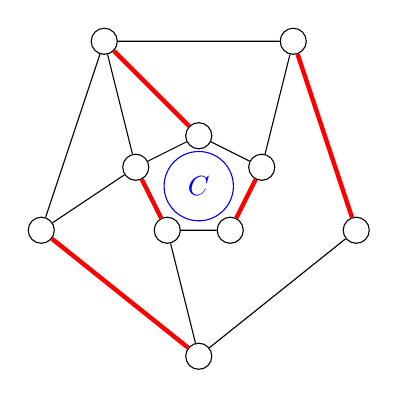
\begin{tikzpicture}[scale=0.8]
                \begin{scope}[
                        every node/.style={circle, draw}
                    ]

                    \node (o1) at (2.5,0) {};
                    \node (o2) at (5,2) {};
                    \node (o3) at (4,5) {};
                    \node (o4) at (1,5) {};
                    \node (o5) at (0,2) {};

                    \node (i1) at (2,2) {};
                    \node (i2) at (3,2) {};
                    \node (i3) at (3.5,3) {};
                    \node (i4) at (2.5,3.5) {};
                    \node (i5) at (1.5,3) {};
                \end{scope}

                \draw (o1) edge (o2);
                \draw[red, ultra thick] (o2) edge (o3);
                \draw (o3) edge (o4);
                \draw (o4) edge (o5);
                \draw[red, ultra thick] (o5) edge (o1);
                \draw[blue] (2.5,2.7) circle (0.55);
                \node[blue] (C) at (2.5,2.7) {$C$};

                \draw (i1) edge (i2);
                \draw[red, ultra thick] (i2) edge (i3);
                \draw (i3) edge (i4);
                \draw (i4) edge (i5);
                \draw[red, ultra thick] (i5) edge (i1);

                \draw (o1) edge (i1);
                \draw (o3) edge (i3);
                \draw[red, ultra thick] (o4) edge (i4);
                \draw (o4) edge (i5);
                \draw (o5) edge (i5);
            \end{tikzpicture}
        \end{minipage}
        $\overset{\text{shrinking}}{\longrightarrow}$
        \begin{minipage}{0.4\textwidth}
            \centering
            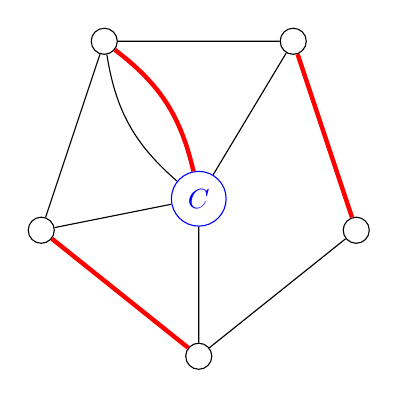
\begin{tikzpicture}[scale=0.8]
                \begin{scope}[
                        every node/.style={circle, draw},
                        every edge/.style={draw, semithick}
                    ]

                    \node (o1) at (2.5,0) {};
                    \node (o2) at (5,2) {};
                    \node (o3) at (4,5) {};
                    \node (o4) at (1,5) {};
                    \node (o5) at (0,2) {};

                    \node[draw=blue, text=blue] (c) at (2.5,2.5) {$C$};
                \end{scope}

                \draw (o1) edge (o2);
                \draw[red, ultra thick] (o2) edge (o3);
                \draw (o3) edge (o4);
                \draw (o4) edge (o5);
                \draw[red, ultra thick] (o5) edge (o1);


                \draw (o1) edge (c);
                \draw (o3) edge (c);
                \draw[red, ultra thick] (o4) edge[bend left=20] (c);
                \draw (o4) edge[bend right=20] (c);
                \draw (o5) edge (c);
                % \end{scope}
            \end{tikzpicture}
        \end{minipage}
    \end{minipage}
    \vspace{5pt}
    \\
    Additionally, a matching \textcolor{red}{$M'$} in the shrinked graph and its corresponding
    extended matching \textcolor{red}{$M$} in the original graph is shown.
\end{example}
\begin{observe}
    The number of $M'$-exposed nodes in $G'$ is retained by the extended matching $M$.
\end{observe}
\begin{warning}
    By this procedure, it is generally \emph{not} true that $M$ is maximum iff $M'$ is maximum.
    Therefore, we need to circumvent this issue in order to use this fact.
\end{warning}
\begin{theorem}
    Given $G,M$, and an odd cycle $C$ such that
    \begin{align*}
        |M \cap C| = \frac{|C|-1}{2}.
    \end{align*}
    Let $c \in C$ be the one not covered within $C$. Suppose that for any $M$-exposed
    node $r$, all alternating $r-c$-paths are disjoint from $V(C)-c$.

    Then, $M$ is maximum in $G$ iff $M'$ is maximum in $G'$.
\end{theorem}
\begin{example}
    Following graphs illustrate when the conditions of the theorem hold and do not hold for some matching $\textcolor{red}{M}$,
    with a bad \textcolor{blue}{$r-c$-path}.
    \vspace{8pt}
    \\
    \begin{minipage}{\textwidth}
        \centering
        \begin{minipage}{0.4\textwidth}
            \centering
            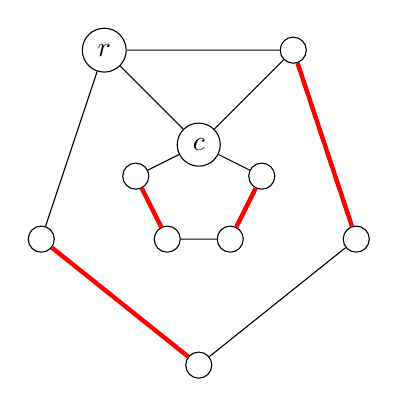
\begin{tikzpicture}[scale=0.8]
                \begin{scope}[
                        every node/.style={circle, draw}
                    ]

                    \node (o1) at (2.5,0) {};
                    \node (o2) at (5,2) {};
                    \node (o3) at (4,5) {};
                    \node (o4) at (1,5) {$r$};
                    \node (o5) at (0,2) {};

                    \node (i1) at (2,2) {};
                    \node (i2) at (3,2) {};
                    \node (i3) at (3.5,3) {};
                    \node (i4) at (2.5,3.5) {$c$};
                    \node (i5) at (1.5,3) {};
                \end{scope}

                \draw (o1) edge (o2);
                \draw[red, ultra thick] (o2) edge (o3);
                \draw (o3) edge (o4);
                \draw (o4) edge (o5);
                \draw[red, ultra thick] (o5) edge (o1);

                \draw (i1) edge (i2);
                \draw[red, ultra thick] (i2) edge (i3);
                \draw (i3) edge (i4);
                \draw (i4) edge (i5);
                \draw[red, ultra thick] (i5) edge (i1);

                % \draw (o1) edge (i1);
                \draw (o3) edge (i4);
                \draw (o4) edge (i4);
                % \draw (o4) edge (i5);
                % \draw (o5) edge (i5);
            \end{tikzpicture}
        \end{minipage}
        vs.
        \begin{minipage}{0.4\textwidth}
            \centering
            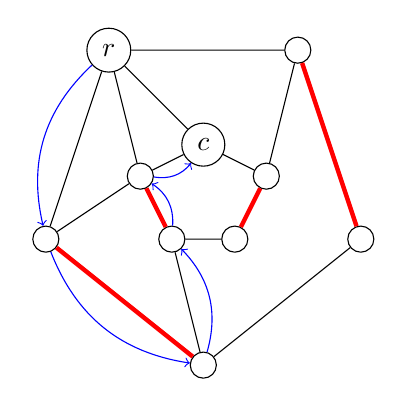
\begin{tikzpicture}[scale=0.8]
                \begin{scope}[
                        every node/.style={circle, draw}
                    ]

                    \node (o1) at (2.5,0) {};
                    \node (o2) at (5,2) {};
                    \node (o3) at (4,5) {};
                    \node (o4) at (1,5) {$r$};
                    \node (o5) at (0,2) {};

                    \node (i1) at (2,2) {};
                    \node (i2) at (3,2) {};
                    \node (i3) at (3.5,3) {};
                    \node (i4) at (2.5,3.5) {$c$};
                    \node (i5) at (1.5,3) {};
                \end{scope}

                \draw (o1) edge (o2);
                \draw[red, ultra thick] (o2) edge (o3);
                \draw (o3) edge (o4);
                \draw (o4) edge (o5);
                \draw[red, ultra thick] (o5) edge (o1);

                \draw (i1) edge (i2);
                \draw[red, ultra thick] (i2) edge (i3);
                \draw (i3) edge (i4);
                \draw (i4) edge (i5);
                \draw[red, ultra thick] (i5) edge (i1);

                \draw (o1) edge (i1);
                \draw (o3) edge (i3);
                \draw (o4) edge (i4);
                \draw (o4) edge (i5);
                \draw (o5) edge (i5);

                \draw[blue,->] (o4) edge [bend right=30](o5);
                \draw[blue,->] (o5) edge [bend right=30](o1);
                \draw[blue,->] (o1) edge [bend right=30](i1);
                \draw[blue,->] (i1) edge [bend right=30](i5);
                \draw[blue,->] (i5) edge [bend right=30](i4);
            \end{tikzpicture}
        \end{minipage}
    \end{minipage}
\end{example}
\begin{proof}
    First, suppose $M$ is maximum, but $M'$ is not. Then $|M'|=|M|-k$ with
    \begin{align*}
        k \coloneqq |M \cap C| = \frac{|C|-1}{2}.
    \end{align*}
    If there exists a matching $N'$ in $G'$ with $|N'|>|M'|$, then there exists a matching $N$ in $G$
    with
    \begin{align*}
        |N| = |N'|+k > |M|
    \end{align*}
    Contradiction!

    For the other direction, suppose $M'$ is maximum, but $M$ is not.
    Then there exists an augmenting path $P$ in $G$.
    Let $v$ be an endnode of $P$ that is not in $V(C)$, and consider two cases:
    \begin{itemize}
        \item $P \cap C = \emptyset$: Let $w$ be the other endnode.
        \item $P \cap C \neq \emptyset$: Then $P \cap C$ consists only of the unmatched node $c$ inside of $C$,
              otherwise we could construct an alternating $r-c$-path starting from one of the end nodes of $P$.
              Again, let $w$ be the other endnode.
              \todo{ask why script seems wrong}
    \end{itemize}
    As a consequence, the $v-w$-path is $M'$-augmenting - contradiction!
\end{proof}
\begin{algorithm}[H] \label{algo:alt_tree}
    \SetAlgoLined
    Graph $G$, matching $M$, exposed node $r$\\
    $A \leftarrow \emptyset$\\
    $B \leftarrow \{r\}$\\
    \While{for any $w \in V, u \in B, v \not \in A \cup B$: $(u,v)\in E, (v,w)\in M$}{
        $A \leftarrow A + v$\\
        $B \leftarrow B + w$\\
    }
    %  reindeer $\leftarrow$ 0\tcp*{current position of reindeer} 
    \caption{Alternating tree-algorithm}
\end{algorithm} \noindent
\begin{definition}
    The tree we get by this algorithm is called $M$-\vocab{alternating tree}.
\end{definition}
\begin{example}
    An exemplary run of the algorithm with two roots $r_1,r_2$, a \textcolor{red}{matching $M$},
    and one \textcolor{orange}{odd cycle $C$} could yield following alternating forest,
    \vspace{8pt}
    \\
    \begin{minipage}{\textwidth}
        \centering
        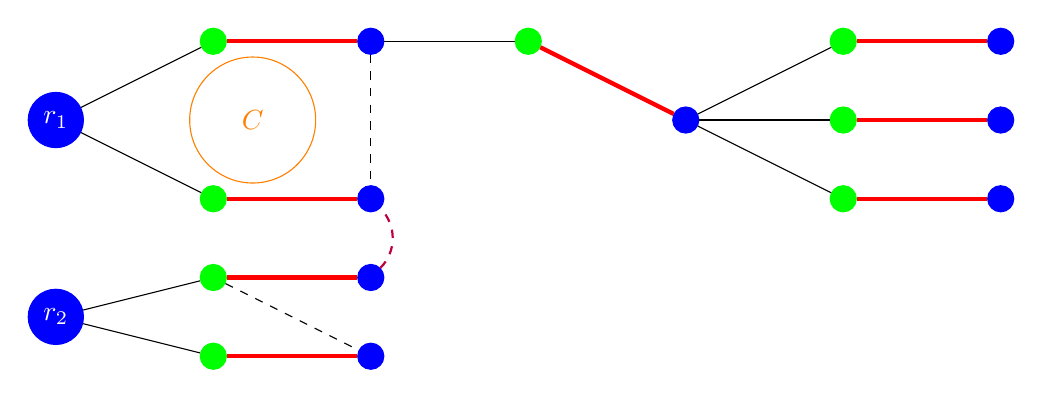
\begin{tikzpicture}
            \begin{scope}[
                    every node/.style={circle, draw=blue, text=white, fill=blue}
                ]

                \node (r) at (0,0) {$r_1$};
                \node (rr) at (0,-2.5) {$r_2$};
                \node (b1) at (4,1) {};
                \node (b2) at (4,-1) {};
                \node (bb1) at (4,-2) {};
                \node (bb2) at (4,-3) {};
                \node (b3) at (8,0) {};
                \node (b4) at (12,1) {};
                \node (b5) at (12,0) {};
                \node (b6) at (12,-1) {};
            \end{scope}
            \begin{scope}[
                    every node/.style={circle, draw=green, fill=green}
                ]
                \node (a1) at (2,1) {};
                \node (a2) at (2,-1) {};
                \node (a3) at (6,1) {};
                \node (a4) at (10,1) {};
                \node (a5) at (10,0) {};
                \node (a6) at (10,-1) {};
                \node (aa1) at (2,-2) {};
                \node (aa2) at (2,-3) {};
            \end{scope}

            \draw[orange] (2.5,0) circle (0.8);
            \node[orange] (C) at (2.5,0) {$C$};

            \draw (r) edge (a1);
            \draw (r) edge (a2);
            \draw (b1) edge (a3);
            \draw (b3) edge (a4);
            \draw (b3) edge (a5);
            \draw (b3) edge (a6);
            \draw (rr) edge (aa1);
            \draw (rr) edge (aa2);

            \draw[dashed] (b1) edge (b2);
            \draw[dashed] (aa1) edge (bb2);
            \draw[dashed, purple, thick] (bb1) edge[bend right=45] (b2);

            \begin{scope}[
                    every edge/.style={draw=red, ultra thick}
                ]
                \draw (a1) edge (b1);
                \draw (a2) edge (b2);
                \draw (a3) edge (b3);
                \draw (a4) edge (b4);
                \draw (a5) edge (b5);
                \draw (a6) edge (b6);
                \draw (aa1) edge (bb1);
                \draw (aa2) edge (bb2);
            \end{scope}

        \end{tikzpicture}
    \end{minipage}
    \vspace{5pt}
    \\
    with \textcolor{green}{$A$} and \textcolor{blue}{$B$} colored correspondingly.
    Non-tree edges are left dashed. The purple edge could be used to connect the two roots.
    (Actually, going from $r_1$, the node colors for the part after this edge should be swapped. Same for $r_2$ the other way round)
\end{example}
\begin{observe} Using this algorithm we see
    \begin{itemize}
        \item $A$ ($B$) contains all nodes that are endnodes of an odd (even)-length $M$-alternating path on $T$,
        \item every node other than $r$ is covered by an edge in $M \cap E(T)$,
        \item every path from $r$ to any $v \in V(T)$ in $T$ is alternating,
        \item $|B|=|A|+1$
    \end{itemize}
    Additionally, we can conclude that any $(u,v) \in E$
    with $u,v \in B$ forms an odd cycle $C$ - shrinking it to node $c$
    (and adding $c$ to $B$) does not affect our structure.

    Finally, if $M$-alternating trees from two roots $r_1, r_2$ share an $(u,v) \in E$ with
    $u \in B_1, v \in B_2$, then there exists an $M$-augmenting path from $r_1$ to $r_2$.
\end{observe}
Now all preliminaries are set to construct the algorithm we long for.

